\documentclass[a4paper]{report}
% Fonte & encodage
\renewcommand{\familydefault}{\sfdefault}
\usepackage[utf8]{inputenc}
%\usepackage[T1]{fontenc}
\usepackage[french]{babel}
\usepackage{color}
% Réduire les marges
%\usepackage{fullpage}
% Pour pouvoir insérer des images
\usepackage{graphicx}
\graphicspath{images/}
% Pour pouvoir insérer des hyperliens
\usepackage{hyperref}

% Ne veut pas afficher le mot 'Chapitre' avant chaque chapitre
\usepackage{titlesec}
\titleformat{\chapter}[hang]{\bf\huge}{\thechapter}{2pc}{}

% ------------------------------------ %
% -- METADONNÉES DU DOCUMENT --------- %
% Utilisées pour générer la page de garde
\title{
	Quelles solutions pour le droit d'auteur à l'ère d'Internet ?\\
	Projet Personnel en Humanités, INSA Lyon
}
\author{Merlin Nimier-David}
\date{Mai 2014}

\begin{document}

	% Génération de la page de garde
	\maketitle

	% Génération de la table des matières
	\tableofcontents

	\chapter{TODO}
	\begin{enumerate}
		\item Bibliographie \cite{hellobib14} (fichier \texttt{.bib})
		\item Source de chaque figure
		\item Remplacer les titres ``in picture'' par des \texttt{caption}
		\item Remplacer les footnotes (``Source : '') par des références de la bibliographie.
		\item Insérer des images d'agrément
		\item Bien centrer les graphiques
		\item Actualiser la partie \ref{declin-systeme} (Système sur le déclin) : l'industrie musicale atteint l'équilibre grâce aux achats numériques (citer le podcast — Pascal Nègre)
	\end{enumerate}


	% ///////////////////////////////////////////////////////// %
	% /// INTRODUCTION //////////////////////////////////////// %
	\chapter{Introduction}
	Il n'a jamais été aussi facile d'accéder à une œuvre qu'aujourd'hui. Sans connaissance technique particulière et simplement équipé d'un accès à internet, n'importe que morceau de musique est accessible. Cette affirmation est également vraie pour les films, séries, livres, jeux vidéo et logiciels. L'accès universel à la culture a changé notre manière de la percevoir — tout du moins en ce qui concerne les \emph{digital natives}. Cette culture est désormais réellement \emph{populaire}, c'est-à-dire accessible à tous, sans barrière financière. Mais comment assurer la pérennité économique d'une industrie entière alors que ses produits pourraient avoir perdu toute valeur monétaire aux yeux de ses consommateurs ?

	Nous adoptons ici un point de vue économique centré sur la question du droit d'auteur, laissant volontairement de côté les aspects juridiques ou éthiques associés. De même, on se concentrera sur les œuvre enregistrées et distribuables et n'inclurons donc pas le spectacle vivant, les peintures, sculptures, etc. En première partie, nous présentons une vue simplifiée du marché de la culture et donnons un historique rapide de son évolution récente. Nous abordons ensuite les solutions ayant été expérimentées. Enfin, nous tenterons de mettre en avant plusieurs solutions alternatives.

	% ///////////////////////////////////////////////////////// %




	% ///////////////////////////////////////////////////////// %
	% /// ÉVOLUTION /////////////////////////////////////////// %
	\chapter{Évolution générale du marché de la culture}
	
	% ------------------------------------ %
	% -- ORGANISATION -------------------- %
	\section{Vue simplifiée de l'industrie culturelle}

	\begin{figure}[ht]
		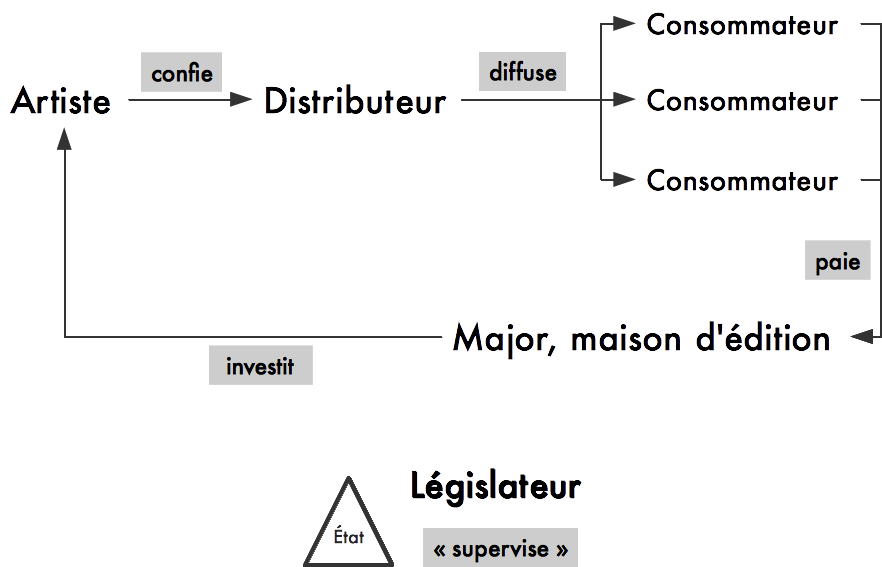
\includegraphics[width=13cm]{images/organisation-industrie-culturelle.png}
		\caption{Vue simplifiée de l'organisation de l'industrie culturelle}
	\end{figure}

	Au moment de sa forte croissance et de l'émergence des majors, l'industrie de la musique s'est organisée en un système bien réglé. Nous dépeignons une version simplifiée du parcours d'une œuvre quelconque : que l'on parle d'un morceau de musique, films, séries, livres, jeux vidéo ou logiciels, le schéma reste presque identique.\\

	Tout d'abord, l'artiste (ou bien le groupe) produit une œuvre. Pour vivre au jour le jour, ou bien pour couvrir les frais de production, l'artiste peut recevoir une avance sur les recettes futures de la part de sa maison d'édition ou d'une major. L'œuvre est ensuite confiée au distributeur, qui se charge de la vendre aux consommateurs finaux. Ces derniers paient le distributeur pour acquérir un exemplaire physique ou digital. Le distributeur reverse de l'argent à la major, qui en redistribue enfin une part à l'artiste original.\\

	Un des éléments-clés ici est le rôle de producteur qu'assument les majors. En effet, c'est grâce à cet investissement que de jeunes artistes peuvent tenter une percée dans le grand public. Cet investissement permet notamment de couvrir les frais d'enregistrement et de communication, qui auraient sinon étés rédhibitoires. Lorsque les majors se sentent financièrement fragiles, elles se replient en toute logique vers les investissements les plus sûrs. Ce sont donc les artistes les plus originaux ou ``risqués'' qui subissent le manque à gagner des majors.\\

	On remarque bien que les intérêts de chacun de ces acteurs diffèrent. Les majors et distributeurs sont des sociétés privées : elles visent avant tout une forte rentabilité. On peut supposer que l'artiste souhaite vivre de son travail et toucher un public le plus grand possible. Le consommateur veut écouter la musique de ses groupes préférés, suivre les séries qu'il aime, etc ; ceci instantanément et à moindre coût. Le législateur, quand à lui, veille à ce que le schéma soit respecté – plus globalement, il s'assure que l'économie reste active.

	\begin{figure}[ht]
		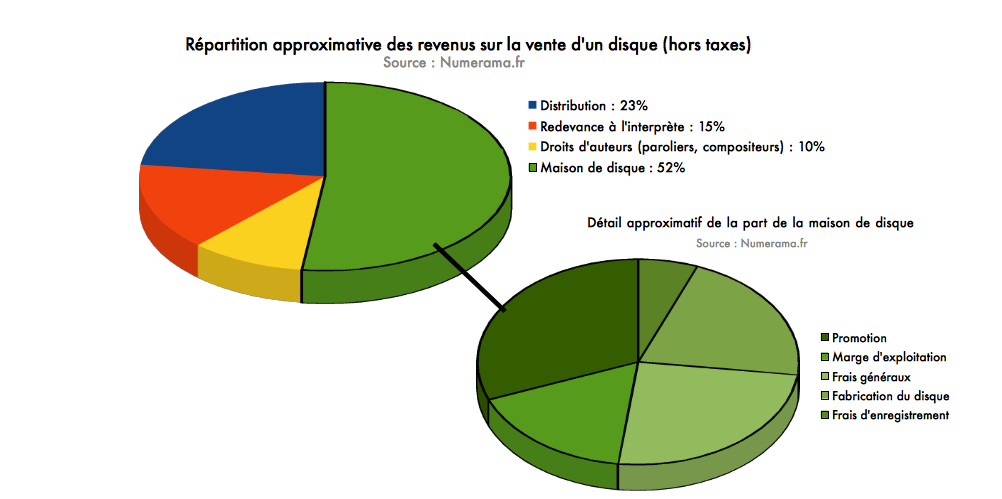
\includegraphics[width=13cm]{images/repartition-des-revenus.png}
		\caption{Répartition moyenne des revenus sur la vente d'un disque (hors taxes)}
	\end{figure}

	Il est important de remarquer qu'avec ce schéma d'organisation, les auteurs se partagent en général 10 à 15\% seulement du prix final payé par le consommateur\footnote{Hors taxes. Source : Epok, un hebdomadaire distribué par la FNAC.}. Ils peuvent cependant, dans une certaine mesure, s'appuyer sur d'autres sources de revenus : les diffusions à la radio ou à la télévision, les concerts, les locations, etc.
	% ------------------------------------ %

	% ------------------------------------ %
	% -- LA RÉVOLUTION NAPSTER ----------- %
	\section{La révolution Napster}
	Depuis l'avènement de l'Internet à haut-débit, la popularité du partage de fichiers est montée en flèche. D'abord réservée à un petit groupe de technophiles fréquentant les \emph{newsgroups}, cette pratique s'est rapidement étendue.

	\begin{figure}[ht]
		\begin{center}
			
\includegraphics[width=6cm]{images/logos/napster.jpg}
			\caption{Logo de Napster, le premier logiciel de partage \emph{peer-to-peer} populaire}
		\end{center}
	\end{figure}

	En Juin 1999, un véritable pavé est jeté dans la mare de l'industrie culturelle : Napster. Crée par Shawn Fanning et Sean Parker, ce logiciel basé sur la technologie \emph{peer-to-peer} permettait de partager facilement mais surtout gratuitement des fichiers de musique piratés. Son succès fulgurant poussa les majors à porter plainte pour violation massive du droit d'auteur, et le service fut fermé en juillet 2001\footnote{Source : Wikipédia [\href{http://fr.wikipedia.org/wiki/Napster}{fr.wikipedia.org/wiki/Napster}].}.\\

	Cependant, ce logiciel pionnier a inspiré la création de nombreux produits aux services similaires, dont une partie existe toujours : Emule, Limewire, Kazaa et Edonkey – pour ne citer que les plus connus. En effet, le service offert (partage de fichiers en utilisant la technologie \emph{peer-to-peer}) n'est pas illégal en soit, puisqu'il peut également servir à distribuer des fichiers libres de droits. Il s'agit par exemple d'un mode de transfert populaire pour les distributions Linux.

	% ------------------------------------ %
	% -- LE TÉLÉCHARGEMENT DIRECT -------- %
	\section{L'avènement du téléchargement direct}
	Depuis la mise en application de la loi Hadopi, qui prévoit la surveillance des réseaux P2P, les amateurs français de téléchargement se sont tournés\footnote{Source : comScore.} vers une solution alternative : le téléchargement direct. Cette technique, plutôt que de mettre à profit l'ensemble des téléchargeurs, établit une connexion directe avec un serveur, qui détient le fichier recherché. Ainsi, des hébergeurs de contenu tels que Mega.co.nz et Rapidshare fournissent les fichiers – souvent piratés – depuis leurs propres serveurs, situés dans des pays n'appliquant pas la réglementation française concernant le droit d'auteur. Bien que le téléchargement lui même soit gratuit pour l'utilisateur, ces entreprises sont financées par la publicité et proposent même un abonnement ``premium'' garantissant une vitesse de téléchargement plus élevée.\\

	Une dernière technologie a vu sa popularité exploser ces dernières années : le \emph{streaming}\footnote{Source : Google Trends.}. Elle permet à l'utilisateur de commencer à regarder une vidéo tout en la téléchargeant ; c'est donc l'outil parfait de consommation instantanée. Utilisée dans un cadre légal par Youtube, Dailymotion et d'autres services d'hébergement de vidéos, elle peut tout aussi bien servir au visionnage de longs-métrages. La démocratisation de son usage – facilitée par des annuaires de liens tels que Allostreaming – a provoqué un grand vent de panique dans l'industrie du cinéma.
	% ------------------------------------ %

	% ------------------------------------ %
	% -- UN SYSTÈME SUR LE DÉCLIN -------- %
	\section{Un système sur le déclin}
	\label{declin-systeme}

	\begin{figure}[ht]
		\begin{center}
			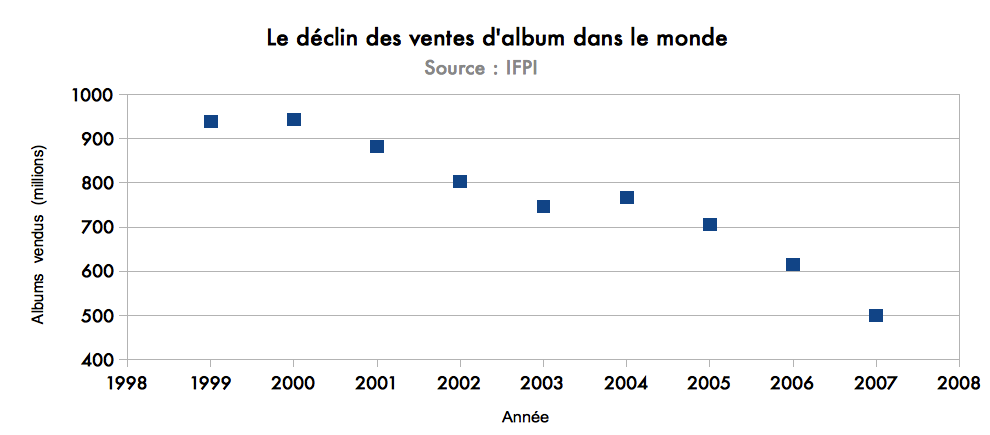
\includegraphics[width=10cm]{images/ventes-albums.png}
			\caption{Le déclin des ventes d'album dans le monde}
		\end{center}
	\end{figure}

	Depuis la banalisation du téléchargement illégal, les ventes de musique sur support physique n'ont cessé de chuter\footnote{Source : IFPI.}. Malgré l'explosion des ventes de musique dématérialisée, le marché reste en baisse. L'industrie du disque est en crise grave et peine à s'adapter aux nouveaux usages. 
	Également touchées, les ventes de DVD: entre 2005 et 2008, le marché français a enregistré une baisse de 30\%\footnote{Source : SEVN.}. Le contraire eut été étonnant : comment le DVD, payant et disponible seulement après six mois d'attente, pourrait se maintenir face à la concurrence du téléchargement illégal, gratuit et disponible parfois même avant la sortie en salles ?\\

	Force est de constater que l'adoption massive du téléchargement illégal a profondément modifié les habitudes des consommateurs. Les jeunes – ces \emph{digital natives} qui constitueront bientôt la majorité du public-cible de l'industrie culturelle – ne sont plus habitués à payer pour de la culture. Dans ce cadre, le schéma présenté plus tôt ne peut se maintenir. Deux alternatives s'ouvrent alors : tenter de ``rétablir l'ordre'' afin de maintenir l'organisation actuelle ou bien réviser ce système et l'adapter aux nouvelles contraintes.
	% ------------------------------------ %

	% ///////////////////////////////////////////////////////// %




	% ///////////////////////////////////////////////////////// %
	% /// LES MESURES EN APPLICATION ////////////////////////// %
	\chapter{Les mesures en application}
	Examiner les différentes solutions mises en place et estimer leur efficacité.

	% ------------------------------------ %
	% -- DES COUPS DE FILET MÉDIATISÉS --- %
	\section{Des coups de filet médiatisés}
	\begin{enumerate}
		\item Allostreaming -$>$ remplaçants
		\item Megaupload -$>$ mega.co.nz (logo, clip, communication)
	\end{enumerate}
	Beaucoup de presse et d'interrogations sur le statut d'hébergeur. Mais solutions de remplacement : lois du marché (demande + faibles barrières à l'entrée =$>$ offre).
	Utilisation de technologies de chiffrement =$>$ ~impossible de bloquer de manière automatique si l'on souhaite respecter le statut d'hébergeur et la neutralité du net.
	% ------------------------------------ %

	% ------------------------------------ %
	% -- TENTATIVES DE RÉGULATION -------- %
	\section{Tentatives de régulation}
	\begin{enumerate}
		\item Échec des DRM
		\item Hadopi
		\item SOPA/PIPA
	\end{enumerate}
	% ------------------------------------ %

	% ------------------------------------ %
	% -- NOUVEAUX MODÈLES ÉCONOMIQUE ----- %
	\section{Nouveaux modèles économique}
	\begin{enumerate}
		\item Distribution numérique (facilité, prix, DRM, pas de hausse de la rémunération malgré les coûts de distribution réduits)
		\item Freemium (Deezer, etc : très faible rémunération)
		\item Offres illimitées
	\end{enumerate}
	% ------------------------------------ %

	% ///////////////////////////////////////////////////////// %




	% ///////////////////////////////////////////////////////// %
	% /// PISTES ALTERNATIVES DE RÉSOLUTION /////////////////// %
	\chapter{Pistes alternatives de résolution}

	\begin{enumerate}
		\item Contournement des majors : explosion du marché indépendant
		\begin{enumerate}
		 	\item financement participatif
		 	\item distribution directe
		 \end{enumerate}
		 \item Diversification de l'offre légale
		 \item Quel rôle pour l'État ? (licence globale ?)
	\end{enumerate}

	% ///////////////////////////////////////////////////////// %




	% ///////////////////////////////////////////////////////// %
	% /// CONCLUSION ////////////////////////////////////////// %
	\chapter{Conclusion}

	Bye.
	% ///////////////////////////////////////////////////////// %



	% Génération de la page de garde
	\bibliographystyle{bibstyle}
	\bibliography{references}




% Fin du document
\end{document}